\documentclass[class=minimal, border = 0pt, crop]{standalone}
\usepackage{pgf}
\usepackage{tikz}
\usepackage[utf8]{inputenc}
\usepackage{amsmath}
\usepackage{amsthm}
\DeclareMathAlphabet\mathbb{U}{msb}{m}{n}
\usetikzlibrary{arrows,automata,shapes,calc,backgrounds,decorations.pathreplacing}
\usetikzlibrary{positioning}
\pagestyle{empty}
\tikzset{
    state/.style={
           rectangle,
           rounded corners,
           draw=black, very thick,
           minimum height=2em,
           inner sep=5pt,
           text centered,
           },
    pil/.style={
           ->,
           thick,
           shorten <=4pt,
           shorten >=4pt,
           },
    ball/.style={
           circle,
           draw,
           align=center,
           anchor=north,
           inner sep=0,
           fill=black,
           }
}

\begin{document}
\centering
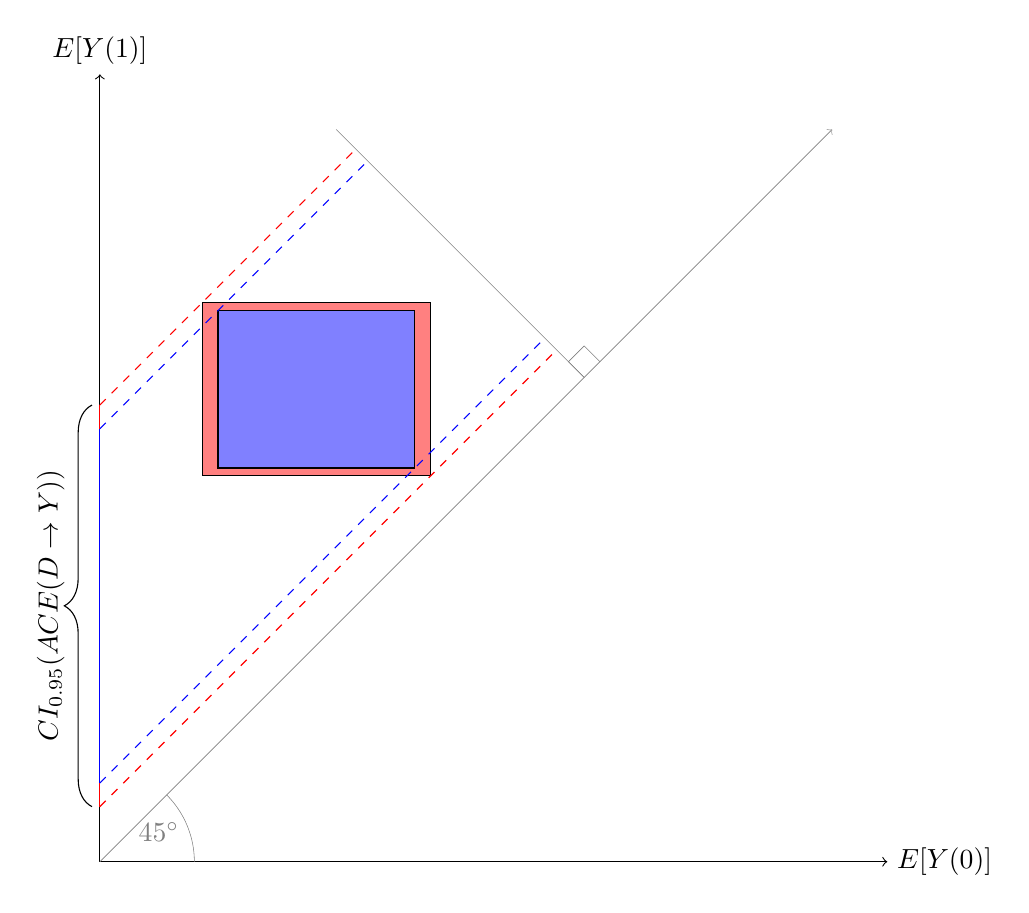
\begin{tikzpicture}
 \coordinate (O) at (0,0);
  \draw[->] (0,0) -- (10,0) coordinate[label = {right:$\mathbb{E}[Y(0)]$}] (xmax);
  \draw[->] (0,0) -- (0,10) coordinate[label = {above:$\mathbb{E}[Y(1)]$}] (ymax);
  \draw[->,help lines] (0,0) -- (9.3,9.3);
  \draw[help lines] (6.15,6.15) -- (5.95,6.35) -- (6.15,6.55) -- (6.35,6.35);
  \draw[help lines] (0,0)+(0:1.2) arc(0:45:1.2) ;
  \draw[fill=red!50] (1.3,4.9) rectangle (4.2,7.1);
  \draw[fill=blue!50] (1.5,5) rectangle (4,7);
  \draw[help lines] (6.15,6.15) -- (3,9.3);
  \draw[color=red, dashed] (0,5.8) -- (3.25,9.05);
  \draw[color=red, dashed] (0,0.7) -- (5.8,6.5);
  \draw[color=blue, dashed] (0,5.5) -- (3.4,8.9);
  \draw[color=blue, dashed] (0,1) -- (5.65,6.65);
  \draw[color=blue] (0,1) -- (0,5.5);
  \draw[color=red] (0,0.7) -- (0,1);
  \draw[color=red] (0,5.5) -- (0,5.8);
%  \draw[color=red] (0,5.8) -- (-0.2,5.8);
%  \draw[color=red] (0,0.7) -- (-0.2,0.7);
%  \draw[color=blue] (0,5.5) -- (-0.2,5.5);
%  \draw[color=blue] (0,1) -- (-0.2,1);
  \draw [decorate,decoration={brace,amplitude=10pt},xshift=-0.1cm,yshift=0pt]
(0,0.7) -- (0,5.8);
\node (a) [] at (-0.5,3.25) {};
\node[rotate=90,anchor=center] at (a.west) {$CI_{0.95}(ACE(D\rightarrow Y))$};
\node[gray=50!] at (0.75,0.375) {$45^\circ$};
\end{tikzpicture}
\end{document}